% Patent Application LaTeX Template with AI Prompting Instructions
% This template follows USPTO requirements and includes detailed guidance
% Use this as a starting point for creating professionally formatted patent applications

\documentclass[12pt,letterpaper]{article}

% Essential packages for patent formatting
\usepackage[top=1in, bottom=1in, left=1in, right=1in]{geometry} % Proper margins
\usepackage{setspace} % For 1.5 or double line spacing
\usepackage{times} % Times Roman font (or use \usepackage{helvet} for Arial)
\usepackage{enumitem} % For customizing lists/enumerations in claims
\usepackage{fancyhdr} % For headers
\usepackage{titlesec} % For section formatting
\usepackage{graphicx} % For including drawings
\usepackage{amsmath} % For mathematical equations
\usepackage{amssymb} % For mathematical symbols
\usepackage{physics} % For quantum mechanics notation
\usepackage{braket} % For quantum state notation
\usepackage{tikz} % For drawing TikZ diagrams
\usetikzlibrary{positioning,arrows.meta}

% Set the line spacing to 1.5 (or 2.0 for double spacing)
\onehalfspacing
% \doublespacing  % Uncomment for double spacing

% Configure headers and footers
\pagestyle{fancy}
\fancyhf{} % Clear all headers and footers
\renewcommand{\headrulewidth}{0pt} % Remove header rule
\fancyfoot[C]{\thepage} % Page number at bottom center

% Configure section formatting
\titleformat{\section}
  {\normalfont\bfseries\uppercase}
  {}
  {0em}
  {}
\titlespacing{\section}{0pt}{12pt}{6pt}

% Configure subsection formatting
\titleformat{\subsection}
  {\normalfont\bfseries}
  {}
  {0em}
  {}
\titlespacing{\subsection}{0pt}{12pt}{6pt}

% Custom paragraph format with additional spacing
\setlength{\parindent}{0pt}
\setlength{\parskip}{6pt}

% Custom enumeration for claims
\newlist{patentclaims}{enumerate}{2}
\setlist[patentclaims,1]{label=\arabic*., align=left, leftmargin=2em, itemsep=1em}
\setlist[patentclaims,2]{label=\arabic*., align=left, leftmargin=2em, itemsep=0.5em}

\begin{document}

% ===== TITLE PAGE =====
\begin{center}
\Large\bfseries
SOFTWARE SYSTEM FOR TEMPORAL PROCESSING USING VIRTUAL MULTI-SHELL ARCHITECTURE
\end{center}

\vspace{0.5in}

\vspace{1in}

\section*{CROSS-REFERENCE TO RELATED APPLICATIONS}

This application is related to co-pending U.S. Patent Application titled "SYSTEM AND METHOD FOR TEMPORAL PROCESSING USING MULTI-SHELL ARCHITECTURE WITH CONFIGURABLE COUPLING," filed concurrently herewith, and U.S. Patent Application titled "SYSTEM AND METHOD FOR MULTI-PHOTON DETECTION USING QUANTUM DOT ARRAYS WITH WAVEFUNCTION-GUIDED SPECTRAL SELECTIVITY," filed concurrently herewith, the entire contents of both are hereby incorporated by reference. The software system described herein provides computational methods for configuring, simulating, and operating the temporal shell architectures and quantum detection systems described in the related applications.

\section*{FIELD OF THE INVENTION}

The present invention relates to computational systems for temporal information processing, and more particularly to software methods and algorithms for configuring and simulating virtual multi-shell temporal architectures with programmable parameters. Specifically, the invention pertains to computational methods, data structures, and algorithms for modeling temporal information processing across multiple timescales using virtual temporal shells and their coupling relationships, with applications in both quantum and classical information processing domains.

\section*{BACKGROUND}

In the field of computational temporal information processing, existing software systems face fundamental limitations in their ability to simulate and process temporal information across multiple timescales while maintaining consistency and correlation in the processed data. This challenge exists in both quantum simulation and classical signal processing software, though with different manifestations and computational constraints.

In quantum simulation software, quantum state evolution and temporal processing algorithms typically operate within a narrow band of temporal scales and lack the flexibility to dynamically adjust their computational parameters for different applications. Current quantum simulation approaches are generally optimized for specific timescales and fail to provide unified frameworks that can coherently process temporal information across multiple scales. These software systems generally implement separate computational modules for different temporal domains, resulting in increased computational complexity and potential inconsistencies at the interfaces between temporal domains.

In classical signal processing software, temporal processing algorithms are typically restricted to fixed timescales determined by sampling rates, window sizes, or filter parameters. Modern digital signal processing libraries and neural network frameworks can process information across different timescales, but they typically use separate processing stages with fixed parameters for each temporal domain, lacking a unified algorithmic framework for multi-scale temporal processing.

Moreover, both quantum and classical temporal processing software typically implement fixed computational architectures that constrain their ability to model complex temporal phenomena. They are generally designed with specific applications in mind and cannot be easily reconfigured for different temporal processing tasks through simple parameter adjustments. This limitation becomes particularly significant when attempting to simulate systems that bridge microscopic phenomena with macroscopic temporal structures or when processing information that contains relevant features across widely varying timescales.

Recent theoretical advances have explored nested computational structures for temporal processing, such as those described in hierarchical modeling frameworks, multi-resolution analysis, and temporal logic, but practical software implementations of such structures have been limited by the lack of comprehensive algorithmic frameworks that can maintain coherence across multiple temporal scales. Additionally, the integration of quantum detection principles with temporal processing algorithms remains largely unexplored in software implementations, despite its potential to significantly enhance system performance.

Therefore, there remains a need for a software system that can effectively simulate and process temporal information across multiple timescales, maintain data coherence, and provide the flexibility to adapt to various applications through reconfigurable parameters and computational architectures. Such a system would ideally leverage advanced computational methods to enhance temporal resolution and enable complex correlation analysis in both quantum and classical simulation domains.

\section*{SUMMARY}

The present invention addresses the aforementioned limitations by providing a software system for temporal processing using a virtual multi-shell architecture with configurable coupling parameters. In one aspect, the invention comprises a computational framework implementing virtual temporal shells represented as software objects with programmable attributes, algorithms for simulating inter-shell coupling and information flow, and data processing methods for temporal correlation analysis and state reconstruction.

The software system can be implemented to simulate both quantum and classical domains. In quantum simulation implementations, the virtual temporal shells maintain quantum coherence properties across multiple timescales, enabling applications in quantum information processing that require accurate modeling of quantum states across temporal domains. In classical implementations, the virtual temporal shells maintain signal coherence and correlation across multiple timescales, enabling applications in advanced signal processing, pattern recognition, and computational modeling.

An advantage of the present invention is the ability to computationally simulate temporal processing across multiple timescales simultaneously while maintaining data coherence, whether in quantum or classical domains. Additionally, the invention allows for reconfigurable shell geometries and processing parameters through software interfaces, rather than requiring new algorithmic implementations for each application.

The virtual multi-shell temporal architecture of the present invention can be advantageously combined with quantum detection simulation systems to create integrated software frameworks for temporal-spectral processing with enhanced capabilities for applications ranging from quantum communication simulation to advanced sensing algorithms and machine learning.

In various embodiments, the software system may include configurable numbers of virtual temporal shells arranged in diverse computational geometries, different coupling algorithms between shells, and application-specific optimization methods to enhance performance for particular use cases ranging from human perceptual processing models to advanced quantum measurement simulations.

\section*{BRIEF DESCRIPTION OF THE DRAWINGS}

FIG. 1 is a block diagram illustrating the overall software architecture of the virtual temporal processing system according to an embodiment of the present invention.

FIG. 2 is a schematic diagram depicting the data structure for configurable multi-shell temporal architecture in a hourglass configuration according to an embodiment of the present invention.

FIG. 3 is a schematic diagram showing a linear configuration of the virtual multi-shell temporal architecture.

FIG. 4 is a schematic diagram showing a nested sphere configuration of the virtual multi-shell temporal architecture.

FIG. 5 is a class diagram illustrating the object-oriented structure of a single virtual temporal shell within the multi-shell architecture.

FIG. 6 is a diagram illustrating the parameter data structures and their relationships across multiple virtual temporal shells.

FIG. 7 is a schematic representation of the computational model for interaction between adjacent virtual temporal shells.

FIG. 8 is a flowchart depicting the algorithmic methods for temporal processing using the virtual multi-shell system.

FIG. 9 is a graph showing computational performance characteristics of the virtual multi-shell architecture compared to conventional temporal processing algorithms.

FIG. 10 is a diagram of the software interfaces for configuration and data exchange with the virtual multi-shell architecture.

\section*{DETAILED DESCRIPTION}

The following detailed description refers to the accompanying drawings which form a part of this disclosure. In the drawings, similar symbols typically identify similar components, unless context dictates otherwise. The illustrative embodiments described herein are not meant to be limiting. Other embodiments may be utilized, and other changes may be made, without departing from the spirit or scope of the subject matter presented here.

Referring first to FIG. 1, a software system for virtual temporal processing 100 includes a computational framework for multi-shell temporal architecture 101 connected to a simulation module for wavefunction-guided detection 102 and a data processing module for temporal correlation and state reconstruction 103. The computational framework 101 forms the core processing element of the system and implements multiple virtual temporal shells arranged in a specific computational configuration optimized for multi-scale temporal processing.

The simulation module 102 is computationally coupled to the framework 101 via data interfaces 104 and functions to transform temporal state information from the virtual shells into signals that can be processed by the data processing module 103. The processing module 103 receives signals from the simulation module 102 through data channels 105 and performs temporal correlation analysis and state reconstruction algorithms.

The system 100 further includes a configuration interface 106 that provides methods for setting control parameters for the computational framework 101, and a system controller module 107 programmatically connected to the framework 101, simulation module 102, and processing module 103 via software control interfaces 108. The system controller 107 functions to adjust operational parameters of the entire system, including shell frequencies, coupling strengths, detection sensitivity, and processing algorithms.

The computational framework 101 implements virtual temporal shells as software objects with configurable attributes. Each virtual shell represents a processing domain optimized for a specific timescale, with the object properties determining its temporal response characteristics. The coupling between virtual shells is implemented through algorithmic methods that define how information flows between the temporal domains.

In the exemplary embodiment, the virtual temporal shells are implemented as objects in an object-oriented programming framework. Each shell object contains data structures representing its current state, methods for evolving that state over time, and interface methods for exchanging information with adjacent shells. The shell objects are organized in a computational graph that defines their relationships and information flow pathways.

The mathematical framework underlying the virtual shell implementation can be expressed through computational operators. For quantum implementations, the state of shell $i$ can be represented as:

$$|\Psi_i\rangle = \sum_j \alpha_{i,j} |j_i\rangle$$

where $|j_i\rangle$ represents the $j$-th basis state of the $i$-th shell, and $\alpha_{i,j}$ are complex probability amplitudes stored in the shell object's state data structure.

The computational algorithm governing the dynamics of each individual shell is derived from the quantum mechanical Hamiltonian:

$$H_i = \hbar\omega_i \sum_j j a_j^{(i)\dagger} a_j^{(i)} - i\hbar\gamma_i \sum_j (a_j^{(i)\dagger} a_j^{(i)})^2$$

where $a_j^{(i)\dagger}$ and $a_j^{(i)}$ are creation and annihilation operators for the $j$-th mode of the $i$-th shell.

In software implementation, these quantum mechanical operations are simulated through linear algebra operations on complex vector spaces, with appropriate numerical techniques to ensure accuracy and stability of the simulation.

For classical implementations, the state of each virtual shell is represented as a continuous or discrete signal $s_i(t)$ that evolves according to shell-specific differential equations such as:

$$\frac{d s_i(t)}{dt} = -\gamma_i s_i(t) + \omega_i \mathcal{F}[s_i(t)] + \sum_j \kappa_{ij} s_j(t)$$

where $\mathcal{F}$ represents a nonlinear transformation function that can be tailored to the specific application.

The software system provides multiple pre-defined shell configurations that can be instantiated through the configuration interface. As shown in FIG. 2, the hourglass configuration includes multiple virtual temporal shells arranged in a specific computational pattern that resembles an hourglass. In this configuration, the shells are organized with varying parameters that optimize information flow between adjacent temporal domains.

Alternative configurations are available, as shown in FIG. 3 (linear configuration) and FIG. 4 (nested sphere configuration). The configuration parameters for each arrangement are stored in configuration files or databases that can be loaded at runtime to establish the desired computational architecture.

In operation, the software system 100 functions as follows, as depicted in the flowchart of FIG. 8. First, at step 601, the system is initialized by configuring the virtual multi-shell architecture through loading of appropriate parameter sets. This involves establishing the desired computational geometry, shell frequencies, decay rates, and coupling coefficients for the specific application.

Next, at step 602, temporal information is input to the computational framework through data input interfaces. When temporal events are processed by the framework at step 603, they induce state changes in one or more virtual temporal shells, creating a specific excitation pattern across the computational architecture.

This pattern is then processed by the simulation module at step 604, which applies appropriate transformations to the data. The transformed data is processed by the data processing module at step 605, which performs temporal correlation analysis to identify relationships between events across different timescales.

At step 606, the original temporal state is reconstructed based on the computed excitation pattern and temporal correlations. Finally, at step 607, the reconstructed temporal information is output for use in further processing, analysis, or visualization.

The computational performance characteristics of the virtual multi-shell architecture compared to conventional temporal processing algorithms are illustrated in FIG. 9. The graph shows the temporal resolution as a function of computational complexity for the virtual multi-shell architecture system compared to conventional algorithms with fixed timescale sensitivity. The virtual multi-shell architecture exhibits enhanced resolution across multiple timescales simultaneously with significantly reduced computational complexity compared to separate processing stages for each timescale.

The software system can be implemented in various programming languages and computational environments. High-level implementations may use Python, MATLAB, or Julia for flexibility and rapid development, while performance-critical components may be implemented in C++, CUDA, or specialized quantum computing languages for maximum efficiency.

For deployment in cloud environments, the system can be containerized using technologies such as Docker and orchestrated with Kubernetes to provide scalable processing capabilities. The system also supports distributed computing configurations where different aspects of the temporal processing pipeline can be executed on separate computing nodes for improved performance.

\subsection{Integration with Hardware Systems}

The software system provides interfaces for integration with physical implementations of the multi-shell architecture and quantum detection systems. These interfaces enable the software to serve as:

\begin{itemize}
    \item A simulation environment for designing and optimizing physical implementations
    \item A control system for configuring and operating hardware implementations
    \item A data processing framework for analyzing results from hardware experiments
    \item A development platform for new temporal processing algorithms
\end{itemize}

The integration interfaces use standardized data formats and communication protocols to ensure compatibility with various hardware implementations and third-party software tools.

\subsection{Applications and Use Cases}

The software system enables a wide range of applications across different domains:

\begin{itemize}
    \item Quantum information processing: Simulation of quantum temporal evolution across multiple timescales
    \item Signal processing: Multi-scale temporal analysis of complex signals
    \item Machine learning: Feature extraction across multiple temporal domains
    \item Cognitive modeling: Simulation of hierarchical temporal processing in perception
    \item Financial analysis: Multi-timescale pattern detection in time series data
    \item Scientific computing: Simulation of systems with phenomena occurring at different timescales
\end{itemize}

For each application domain, the system provides domain-specific libraries and configuration templates that optimize the virtual multi-shell architecture for the particular requirements of that domain.

\newpage
\section*{CLAIMS}

\begin{patentclaims}
    \item A computer-implemented method for temporal processing using a virtual multi-shell architecture, the method comprising:
    \begin{itemize}[leftmargin=2em]
        \item instantiating, by a computing device, a plurality of virtual temporal shells arranged in a computational configuration;
        \item configuring processing parameters for each virtual temporal shell to optimize temporal processing across multiple timescales;
        \item establishing computational coupling between adjacent virtual temporal shells;
        \item processing temporal information through the virtual multi-shell architecture; and
        \item performing temporal correlation analysis on the processed information to identify relationships between events across different timescales.
    \end{itemize}
    
    \item The method of claim 1, wherein the computational configuration is selectable from a group consisting of:
    \begin{itemize}[leftmargin=2em]
        \item a linear arrangement;
        \item an hourglass configuration;
        \item a nested sphere configuration; and
        \item arbitrary geometric patterns.
    \end{itemize}
    
    \item The method of claim 1, wherein configuring processing parameters comprises setting for each virtual temporal shell:
    \begin{itemize}[leftmargin=2em]
        \item a base frequency parameter;
        \item a decay rate parameter; and
        \item coupling coefficients with adjacent virtual shells.
    \end{itemize}
    
    \item The method of claim 1, wherein the plurality of virtual temporal shells are implemented as software objects in an object-oriented programming framework, wherein each object includes data structures representing the shell's state and methods for evolving the state over time.
    
    \item The method of claim 1, wherein the method further comprises implementing a quantum simulation of the virtual multi-shell architecture, wherein the processing parameters are derived from quantum mechanical operators.
    
    \item The method of claim 1, wherein the method further comprises implementing a classical simulation of the virtual multi-shell architecture, wherein the processing parameters define differential equations governing the evolution of signals through the virtual shells.
    
    \item The method of claim 1, wherein the computational coupling between adjacent virtual temporal shells is implemented through algorithmic methods that define information flow between temporal domains.
    
    \item The method of claim 1, further comprising:
    \begin{itemize}[leftmargin=2em]
        \item dynamically reconfiguring the virtual multi-shell architecture by adjusting the computational configuration and processing parameters in response to changing processing requirements.
    \end{itemize}
    
    \item The method of claim 1, further comprising:
    \begin{itemize}[leftmargin=2em]
        \item generating control signals for a physical implementation of a multi-shell temporal architecture based on the configured virtual multi-shell architecture.
    \end{itemize}
    
    \item A system for temporal processing comprising:
    \begin{itemize}[leftmargin=2em]
        \item a processor;
        \item a memory coupled to the processor and storing instructions that, when executed by the processor, cause the system to:
        \begin{itemize}
            \item implement a computational framework for a virtual multi-shell temporal architecture comprising a plurality of virtual temporal shells;
            \item implement a simulation module for processing temporal information through the virtual multi-shell architecture; and
            \item implement a data processing module for analyzing temporal correlations in the processed information,
        \end{itemize}
        \item wherein the computational framework maintains coherence of information across multiple timescales.
    \end{itemize}
    
    \item The system of claim 10, wherein the memory further stores instructions for implementing a configuration interface that provides methods for setting control parameters for the computational framework.
    
    \item The system of claim 10, wherein the virtual temporal shells are organized as a computational graph that defines relationships and information flow pathways between the shells.
    
    \item The system of claim 10, wherein the memory further stores instructions for implementing interfaces for integration with physical implementations of multi-shell architecture and quantum detection systems.
    
    \item The system of claim 10, wherein the computational framework implements multiple pre-defined shell configurations that can be instantiated through a configuration interface.
    
    \item The system of claim 10, wherein the memory further stores domain-specific libraries and configuration templates that optimize the virtual multi-shell architecture for particular application domains.
    
    \item A non-transitory computer-readable medium storing instructions that, when executed by a processor, cause the processor to:
    \begin{itemize}[leftmargin=2em]
        \item instantiate a virtual multi-shell temporal architecture comprising a plurality of virtual temporal shells arranged in a configurable computational geometry;
        \item configure shell-specific parameters for each virtual temporal shell, the parameters including base frequency, decay rate, and coupling coefficients;
        \item process temporal information through the virtual multi-shell architecture to enable analysis across multiple timescales simultaneously; and
        \item output processed temporal information for use in quantum simulation, signal processing, or pattern recognition applications.
    \end{itemize}
    
    \item The non-transitory computer-readable medium of claim 16, wherein the instructions further cause the processor to implement a quantum mechanical simulation framework for modeling quantum state evolution across the virtual temporal shells.
    
    \item The non-transitory computer-readable medium of claim 16, wherein the instructions further cause the processor to simulate coupling between adjacent virtual shells using algorithmic representations of quantum mechanical or classical coupling mechanisms.
    
    \item The non-transitory computer-readable medium of claim 16, wherein the instructions further cause the processor to generate visualization outputs showing temporal correlation patterns identified across multiple timescales.
    
    \item The non-transitory computer-readable medium of claim 16, wherein the instructions further cause the processor to optimize computational resources by dynamically allocating processing power to different virtual shells based on detected activity levels.
\end{patentclaims}

\newpage
\section*{ABSTRACT}

A software system for temporal processing using a virtual multi-shell architecture with configurable coupling is disclosed. The system implements computational methods for simulating temporal processing across multiple timescales simultaneously while maintaining data coherence. Virtual temporal shells are implemented as software objects with configurable parameters including base frequency, decay rate, and coupling coefficients. The system supports various computational configurations including hourglass arrangements optimized for human perceptual timescales, linear arrangements for uniform temporal resolution, and nested sphere configurations for three-dimensional spatiotemporal processing. Quantum implementations simulate quantum coherence maintenance and can be integrated with quantum detection simulation systems. Classical implementations simulate signal coherence and can be integrated with conventional signal processing systems. The software system enables advanced temporal correlation analysis with significantly reduced computational complexity compared to conventional temporal processing algorithms. Applications include quantum information processing simulation, multi-scale signal analysis, and temporal pattern recognition across domains ranging from quantum physics to cognitive modeling and financial analysis.

\newpage
\section*{DRAWINGS}

\begin{figure}[h]
\centering
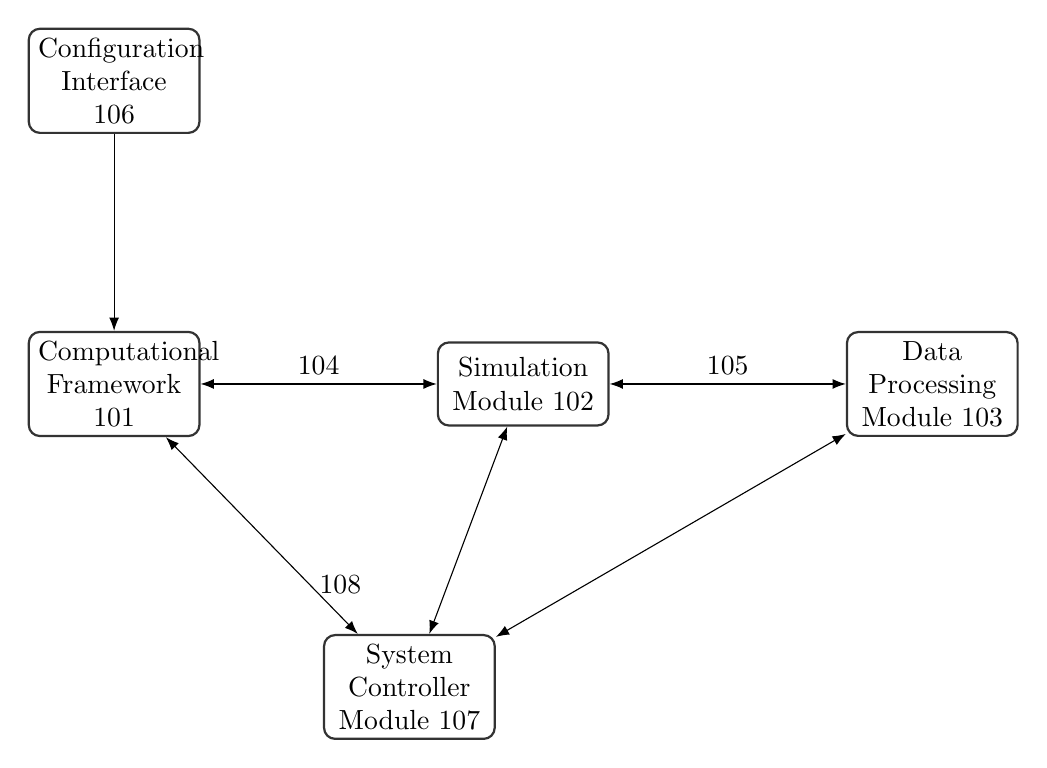
\begin{tikzpicture}[
    node distance=2.5cm and 3cm,
    block/.style={rectangle, draw, fill=white, text width=5.5em, text centered, rounded corners, minimum height=3em},
    mainblock/.style={rectangle, draw, fill=white, text width=5.5em, text centered, rounded corners, minimum height=3em, thick, draw=black!80},
    line/.style={draw, -Latex},
    bidirectional/.style={draw, Latex-Latex},
    scale=1.0
    ]
    
    % Define nodes
    \node[mainblock] (framework) {Computational Framework 101};
    \node[mainblock, right=of framework] (simulation) {Simulation Module 102};
    \node[mainblock, right=of simulation] (processing) {Data Processing Module 103};
    \node[mainblock, above=of framework] (interface) {Configuration Interface 106};
    \node[mainblock, below=of framework, xshift=3.75cm] (controller) {System Controller Module 107};
    
    % Define connections
    \draw[bidirectional] (framework) -- (simulation) node[midway, above] {104};
    \draw[bidirectional] (simulation) -- (processing) node[midway, above] {105};
    \draw[line] (interface) -- (framework);
    \draw[bidirectional] (controller) -- (framework) node[pos=0.25, right] {108};
    \draw[bidirectional] (controller) -- (simulation);
    \draw[bidirectional] (controller) -- (processing);
    
\end{tikzpicture}
\caption*{FIG. 1}
\end{figure}

\begin{figure}[h]
\centering
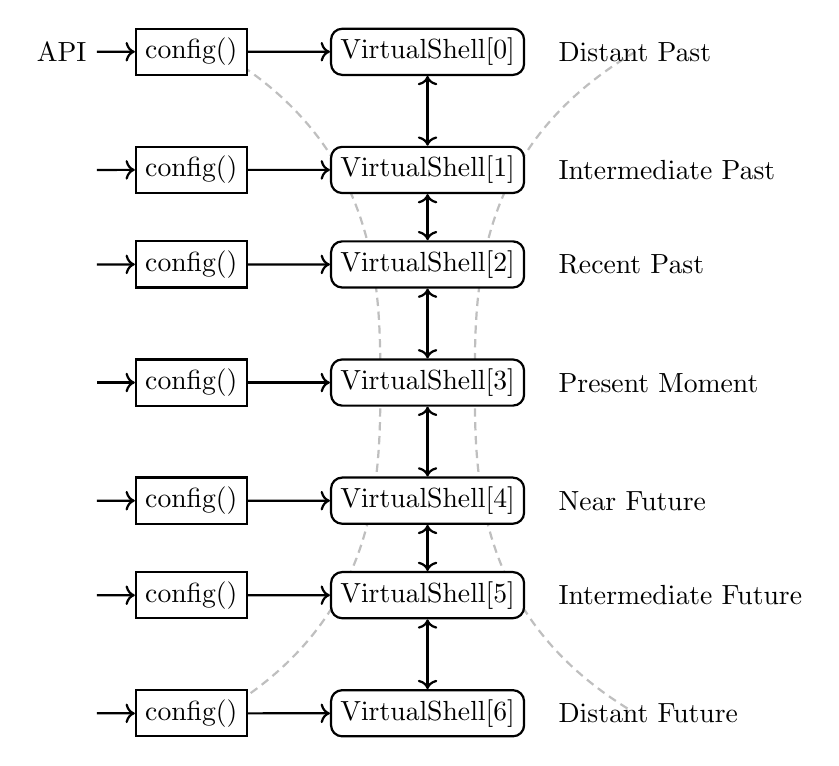
\begin{tikzpicture}[
    scale=1.2,
    shell/.style={rectangle, draw, thick, fill=white, rounded corners},
    control/.style={rectangle, draw, thick, minimum width=0.5cm, minimum height=0.2cm, fill=white},
    connector/.style={thick, ->},
    line/.style={thick}
    ]
    
    % Draw the hourglass shape as a background
    \draw[thick, densely dashed, gray!50] 
        (-2.2,3.5) .. controls (-0.5,2.5) and (-0.5,1) .. (-0.5,0)
        .. controls (-0.5,-1) and (-0.5,-2.5) .. (-2.2,-3.5);
    
    \draw[thick, densely dashed, gray!50] 
        (2.2,3.5) .. controls (0.5,2.5) and (0.5,1) .. (0.5,0)
        .. controls (0.5,-1) and (0.5,-2.5) .. (2.2,-3.5);
    
    % Create shells
    \node[shell] (shell1) at (0,3.5) {VirtualShell[0]};
    \node[shell] (shell2) at (0,2.25) {VirtualShell[1]};
    \node[shell] (shell3) at (0,1.25) {VirtualShell[2]};
    \node[shell] (shell4) at (0,0) {VirtualShell[3]};
    \node[shell] (shell5) at (0,-1.25) {VirtualShell[4]};
    \node[shell] (shell6) at (0,-2.25) {VirtualShell[5]};
    \node[shell] (shell7) at (0,-3.5) {VirtualShell[6]};
    
    % Labels for temporal domains
    \node[right=0.3cm of shell1] {Distant Past};
    \node[right=0.3cm of shell2] {Intermediate Past};
    \node[right=0.3cm of shell3] {Recent Past};
    \node[right=0.3cm of shell4] {Present Moment};
    \node[right=0.3cm of shell5] {Near Future};
    \node[right=0.3cm of shell6] {Intermediate Future};
    \node[right=0.3cm of shell7] {Distant Future};
    
    % Control interfaces for each shell
    \node[control] (control1) at (-2.5,3.5) {config()};
    \node[control] (control2) at (-2.5,2.25) {config()};
    \node[control] (control3) at (-2.5,1.25) {config()};
    \node[control] (control4) at (-2.5,0) {config()};
    \node[control] (control5) at (-2.5,-1.25) {config()};
    \node[control] (control6) at (-2.5,-2.25) {config()};
    \node[control] (control7) at (-2.5,-3.5) {config()};
    
    % Connect controls to shells
    \draw[connector] (control1) -- (shell1);
    \draw[connector] (control2) -- (shell2);
    \draw[connector] (control3) -- (shell3);
    \draw[connector] (control4) -- (shell4);
    \draw[connector] (control5) -- (shell5);
    \draw[connector] (control6) -- (shell6);
    \draw[connector] (control7) -- (shell7);
    
    % Control lines going off to the left
    \draw[line, <-] (control1) -- ++(-1,0) node[left] {API};
    \draw[line, <-] (control2) -- ++(-1,0);
    \draw[line, <-] (control3) -- ++(-1,0);
    \draw[line, <-] (control4) -- ++(-1,0);
    \draw[line, <-] (control5) -- ++(-1,0);
    \draw[line, <-] (control6) -- ++(-1,0);
    \draw[line, <-] (control7) -- ++(-1,0);
    
    % Coupling between shells
    \draw[line, <->] (shell1) -- (shell2);
    \draw[line, <->] (shell2) -- (shell3);
    \draw[line, <->] (shell3) -- (shell4);
    \draw[line, <->] (shell4) -- (shell5);
    \draw[line, <->] (shell5) -- (shell6);
    \draw[line, <->] (shell6) -- (shell7);
    
\end{tikzpicture}
\caption*{FIG. 2}
\end{figure}

\begin{figure}[h]
\centering
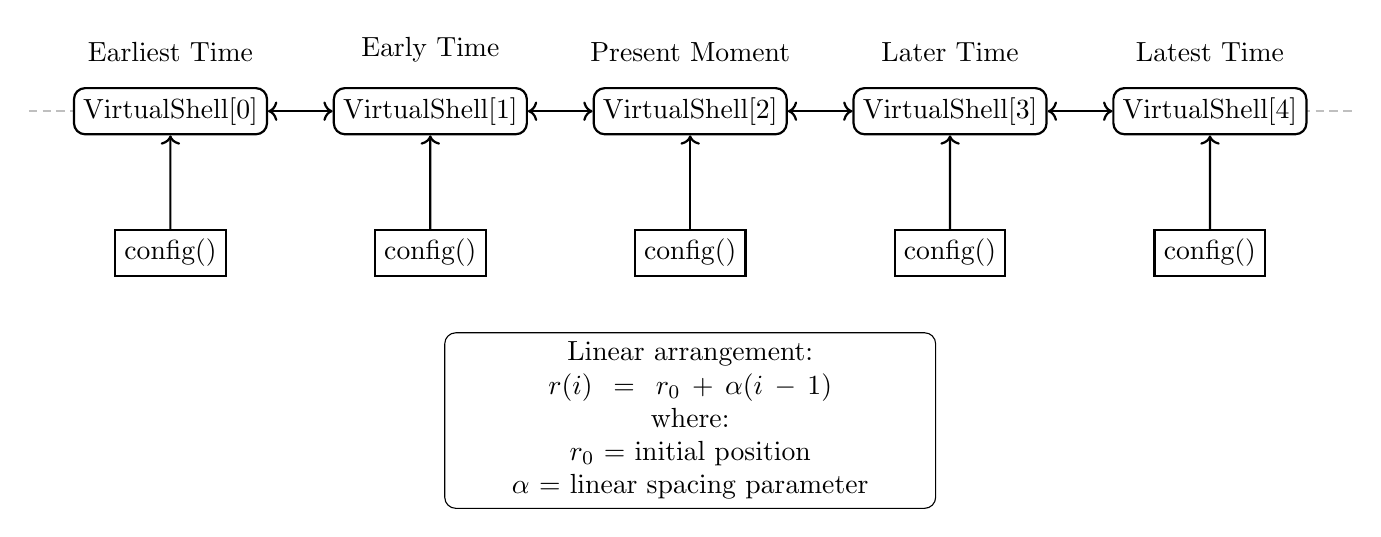
\begin{tikzpicture}[
    scale=1.2,
    shell/.style={rectangle, draw, thick, fill=white, rounded corners},
    control/.style={rectangle, draw, thick, minimum width=0.5cm, minimum height=0.2cm, fill=white},
    connector/.style={thick, ->},
    line/.style={thick}
    ]
    
    % Draw linear background
    \draw[thick, densely dashed, gray!50] (-7,0) -- (7,0);
    
    % Create shells
    \node[shell] (shell1) at (-5.5,0) {VirtualShell[0]};
    \node[shell] (shell2) at (-2.75,0) {VirtualShell[1]};
    \node[shell] (shell3) at (0,0) {VirtualShell[2]};
    \node[shell] (shell4) at (2.75,0) {VirtualShell[3]};
    \node[shell] (shell5) at (5.5,0) {VirtualShell[4]};
    
    % Labels for temporal domains
    \node[above=0.2cm of shell1] {Earliest Time};
    \node[above=0.2cm of shell2] {Early Time};
    \node[above=0.2cm of shell3] {Present Moment};
    \node[above=0.2cm of shell4] {Later Time};
    \node[above=0.2cm of shell5] {Latest Time};
    
    % Control interfaces for each shell
    \node[control] (control1) at (-5.5,-1.5) {config()};
    \node[control] (control2) at (-2.75,-1.5) {config()};
    \node[control] (control3) at (0,-1.5) {config()};
    \node[control] (control4) at (2.75,-1.5) {config()};
    \node[control] (control5) at (5.5,-1.5) {config()};
    
    % Connect controls to shells
    \draw[connector] (control1) -- (shell1);
    \draw[connector] (control2) -- (shell2);
    \draw[connector] (control3) -- (shell3);
    \draw[connector] (control4) -- (shell4);
    \draw[connector] (control5) -- (shell5);
    
    % Coupling between shells
    \draw[line, <->] (shell1) -- (shell2);
    \draw[line, <->] (shell2) -- (shell3);
    \draw[line, <->] (shell3) -- (shell4);
    \draw[line, <->] (shell4) -- (shell5);
    
    % Mathematical formula
    \node[draw, rounded corners, fill=white, text width=6cm, align=center, below=2.5cm of shell3] 
    {Linear arrangement:\\
    $r(i) = r_0 + \alpha(i-1)$\\
    where:\\
    $r_0$ = initial position\\
    $\alpha$ = linear spacing parameter};
    
\end{tikzpicture}
\caption*{FIG. 3}
\end{figure}

\begin{figure}[h]
\centering
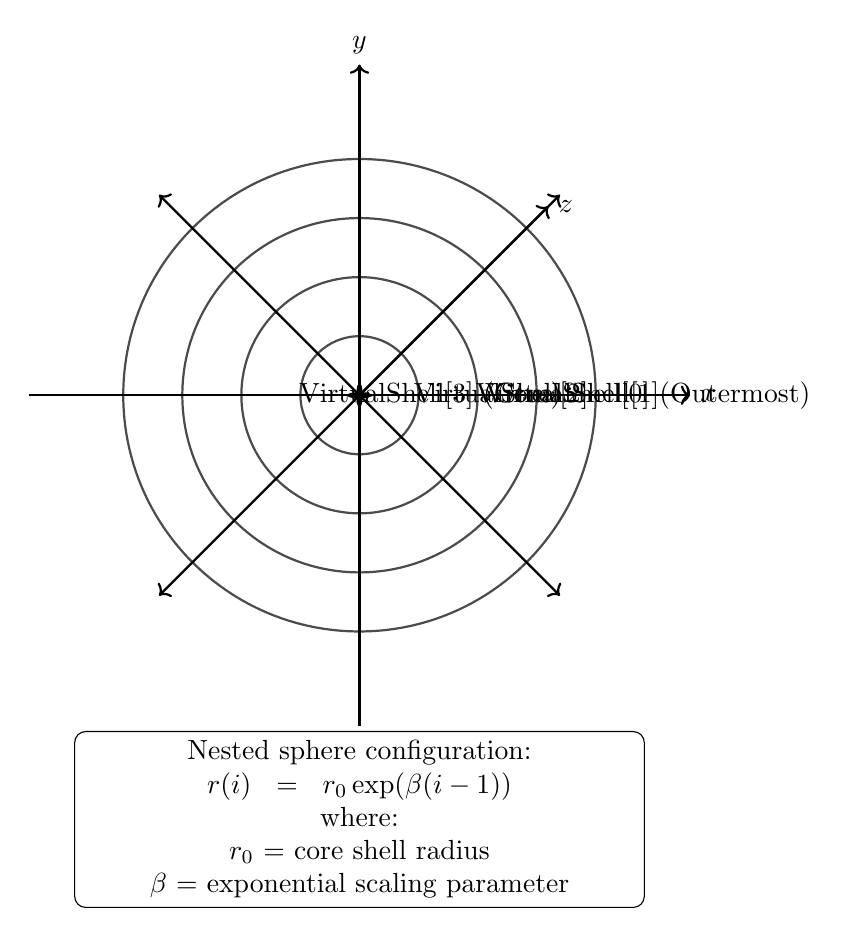
\begin{tikzpicture}[
    scale=1.2,
    shell/.style={circle, draw, thick, fill=white, opacity=0.7},
    connection/.style={thick, <->},
    ]
    
    % Create nested spherical shells
    \node[shell, minimum size=6cm] (shell1) at (0,0) {};
    \node[shell, minimum size=4.5cm] (shell2) at (0,0) {};
    \node[shell, minimum size=3cm] (shell3) at (0,0) {};
    \node[shell, minimum size=1.5cm] (shell4) at (0,0) {};
    
    % Label the shells
    \node at (3.0, 0) {VirtualShell[0] (Outermost)};
    \node at (2.25, 0) {VirtualShell[1]};
    \node at (1.5, 0) {VirtualShell[2]};
    \node at (0.75, 0) {VirtualShell[3] (Core)};
    
    % Draw radial connectors between shells
    \draw[connection] (0,0) -- (45:3);
    \draw[connection] (0,0) -- (135:3);
    \draw[connection] (0,0) -- (225:3);
    \draw[connection] (0,0) -- (315:3);
    
    % Add some coordinate axes
    \draw[->, thick] (-3.5,0) -- (3.5,0) node[right] {$x$};
    \draw[->, thick] (0,-3.5) -- (0,3.5) node[above] {$y$};
    \draw[->, thick] (0,0) -- (2,2) node[right] {$z$};
    
    % Mathematical formula
    \node[draw, rounded corners, fill=white, text width=7cm, align=center, below=3.5cm of shell4] 
    {Nested sphere configuration:\\
    $r(i) = r_0 \exp(\beta (i-1))$\\
    where:\\
    $r_0$ = core shell radius\\
    $\beta$ = exponential scaling parameter};
    
\end{tikzpicture}
\caption*{FIG. 4}
\end{figure}

\begin{figure}[h]
\centering
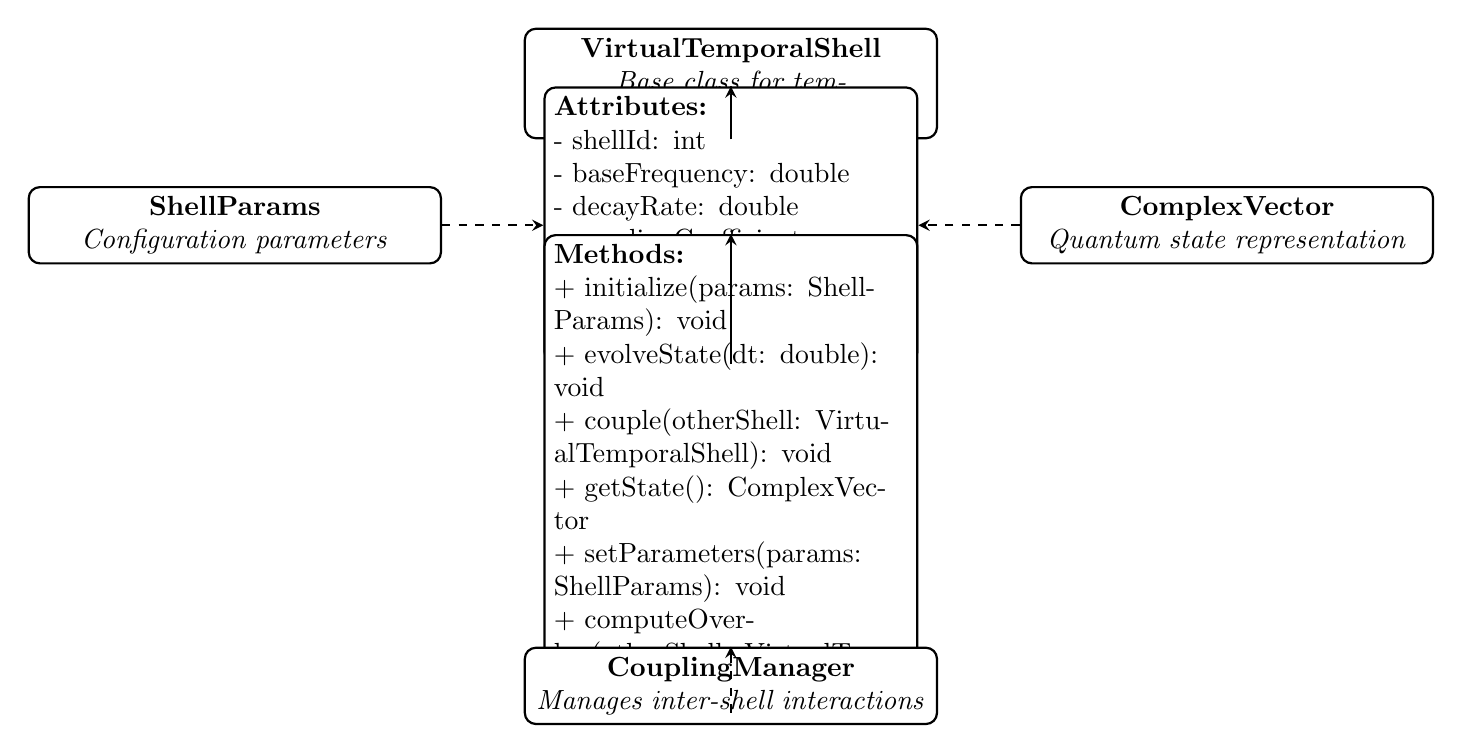
\begin{tikzpicture}[
    scale=0.9,
    class/.style={rectangle, draw, thick, fill=white, text width=5cm, align=center, rounded corners},
    method/.style={rectangle, draw, thick, fill=white!80, text width=4.5cm, align=left, rounded corners},
    attribute/.style={rectangle, draw, thick, fill=white!90, text width=4.5cm, align=left, rounded corners},
    arrow/.style={->, >=stealth, thick},
    ]
    
    % Main class
    \node[class] (shell) at (0,0) {
        \textbf{VirtualTemporalShell}\\
        \emph{Base class for temporal shell objects}
    };
    
    % Attributes section
    \node[attribute] (attributes) at (0,-2) {
        \textbf{Attributes:}\\
        - shellId: int\\
        - baseFrequency: double\\
        - decayRate: double\\
        - couplingCoefficients: Map<int, double>\\
        - state: ComplexVector\\
        - temporalDomain: enum
    };
    
    % Methods section
    \node[method] (methods) at (0,-5.5) {
        \textbf{Methods:}\\
        + initialize(params: ShellParams): void\\
        + evolveState(dt: double): void\\
        + couple(otherShell: VirtualTemporalShell): void\\
        + getState(): ComplexVector\\
        + setParameters(params: ShellParams): void\\
        + computeOverlap(otherShell: VirtualTemporalShell): double
    };
    
    % Connect sections
    \draw[arrow] (shell) -- (attributes);
    \draw[arrow] (attributes) -- (methods);
    
    % Related classes
    \node[class] (params) at (-7,-2) {
        \textbf{ShellParams}\\
        \emph{Configuration parameters}
    };
    
    \node[class] (state) at (7,-2) {
        \textbf{ComplexVector}\\
        \emph{Quantum state representation}
    };
    
    \node[class] (coupling) at (0,-8.5) {
        \textbf{CouplingManager}\\
        \emph{Manages inter-shell interactions}
    };
    
    % Connect related classes
    \draw[arrow, dashed] (params) -- (attributes);
    \draw[arrow, dashed] (state) -- (attributes);
    \draw[arrow, dashed] (methods) -- (coupling);
    
\end{tikzpicture}
\caption*{FIG. 5}
\end{figure}

\begin{figure}[h]
\centering
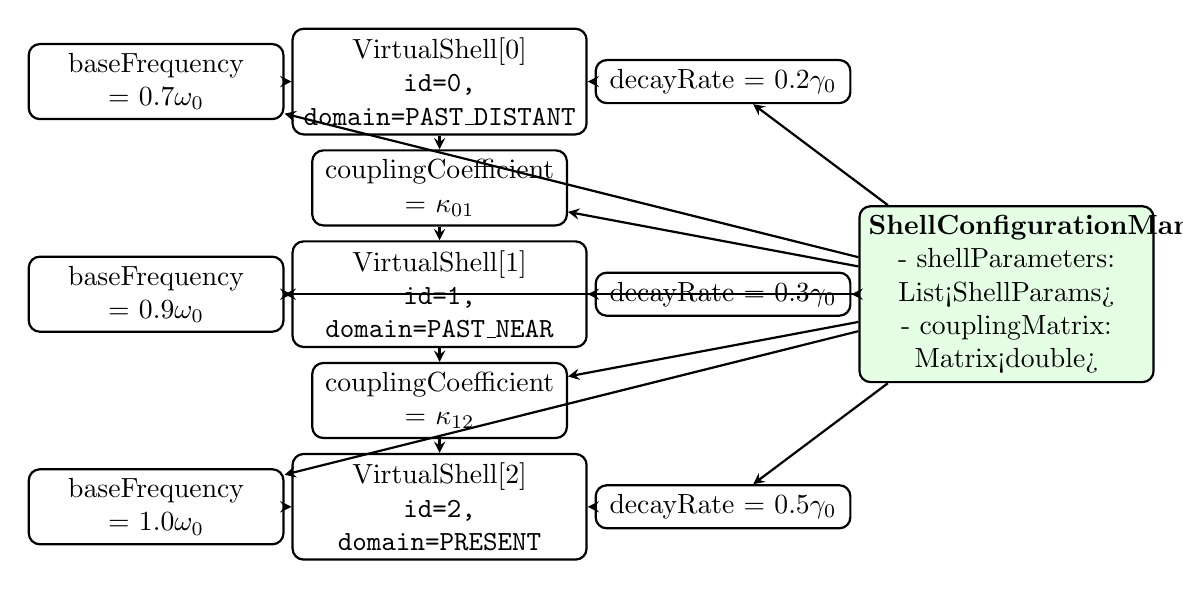
\begin{tikzpicture}[
    scale=0.9,
    param/.style={rectangle, draw, thick, fill=white!90, rounded corners, text width=3cm, align=center},
    shell/.style={rectangle, draw, thick, fill=white, rounded corners, text width=3.5cm, align=center},
    arrow/.style={->, >=stealth, thick},
    relation/.style={->, >=stealth, thick, dashed},
    ]
    
    % Shell objects
    \node[shell] (shell1) at (0,0) {VirtualShell[0]\\ \texttt{id=0, domain=PAST\_DISTANT}};
    \node[shell] (shell2) at (0,-3) {VirtualShell[1]\\ \texttt{id=1, domain=PAST\_NEAR}};
    \node[shell] (shell3) at (0,-6) {VirtualShell[2]\\ \texttt{id=2, domain=PRESENT}};
    
    % Parameters for shell 1
    \node[param] (freq1) at (-4,0) {baseFrequency = 0.7$\omega_0$};
    \node[param] (decay1) at (4,0) {decayRate = 0.2$\gamma_0$};
    
    % Parameters for shell 2
    \node[param] (freq2) at (-4,-3) {baseFrequency = 0.9$\omega_0$};
    \node[param] (decay2) at (4,-3) {decayRate = 0.3$\gamma_0$};
    
    % Parameters for shell 3
    \node[param] (freq3) at (-4,-6) {baseFrequency = 1.0$\omega_0$};
    \node[param] (decay3) at (4,-6) {decayRate = 0.5$\gamma_0$};
    
    % Coupling parameters
    \node[param] (coupling12) at (0,-1.5) {couplingCoefficient = $\kappa_{01}$};
    \node[param] (coupling23) at (0,-4.5) {couplingCoefficient = $\kappa_{12}$};
    
    % Connect shells to their parameters
    \draw[arrow] (freq1) -- (shell1);
    \draw[arrow] (decay1) -- (shell1);
    \draw[arrow] (freq2) -- (shell2);
    \draw[arrow] (decay2) -- (shell2);
    \draw[arrow] (freq3) -- (shell3);
    \draw[arrow] (decay3) -- (shell3);
    
    % Connect shells with coupling parameters
    \draw[relation] (shell1) -- (coupling12);
    \draw[relation] (coupling12) -- (shell2);
    \draw[relation] (shell2) -- (coupling23);
    \draw[relation] (coupling23) -- (shell3);
    
    % Config object
    \node[shell, fill=green!10] (config) at (8,-3) {
        \textbf{ShellConfigurationManager}\\
        - shellParameters: List<ShellParams>\\
        - couplingMatrix: Matrix<double>
    };
    
    % Connect config to all parameters
    \draw[arrow, bend left=10] (config) -- (freq1);
    \draw[arrow, bend left=20] (config) -- (decay1);
    \draw[arrow] (config) -- (freq2);
    \draw[arrow] (config) -- (decay2);
    \draw[arrow, bend right=10] (config) -- (freq3);
    \draw[arrow, bend right=20] (config) -- (decay3);
    \draw[arrow, bend left=45] (config) -- (coupling12);
    \draw[arrow, bend right=45] (config) -- (coupling23);
    
\end{tikzpicture}
\caption*{FIG. 6}
\end{figure}

\begin{figure}[h]
\centering
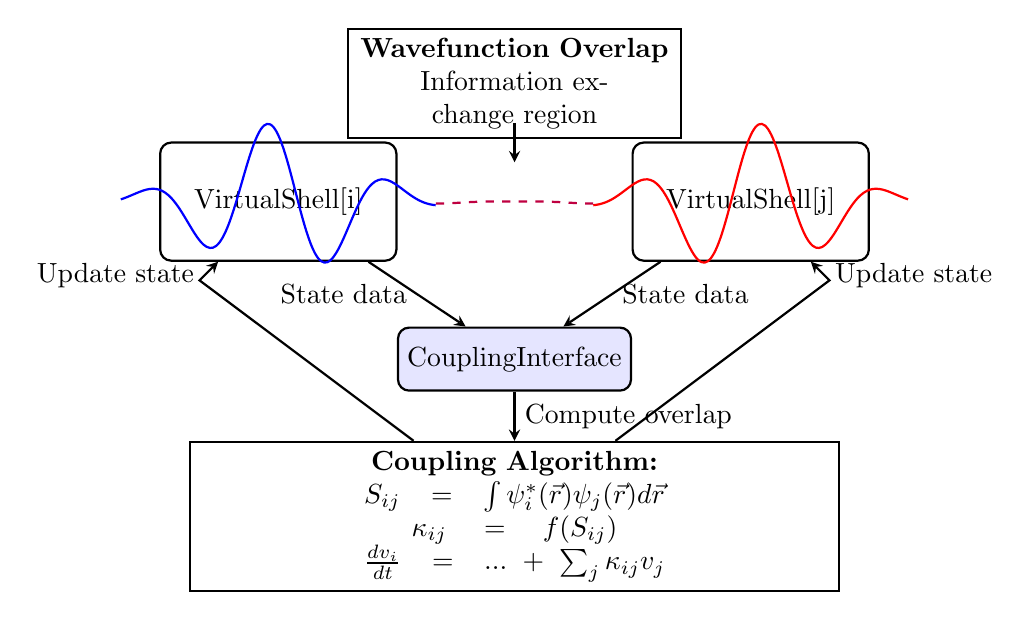
\begin{tikzpicture}[
    scale=1.0,
    shell/.style={rectangle, draw, thick, fill=white, rounded corners, minimum width=3cm, minimum height=1.5cm},
    wave/.style={thick, smooth},
    interface/.style={rectangle, draw, thick, fill=blue!10, rounded corners, minimum width=2cm, minimum height=0.8cm},
    arrow/.style={->, >=stealth, thick},
    ]
    
    % Define shell positions
    \node[shell] (shell1) at (-3,0) {VirtualShell[i]};
    \node[shell] (shell2) at (3,0) {VirtualShell[j]};
    
    % Draw the wavefunction from shell 1
    \draw[wave, blue] plot[domain=-5:-1, samples=100] 
        (\x, {exp(-(\x+3)*(\x+3)/1.5)*cos(4*\x r)});
    
    % Draw the wavefunction from shell 2
    \draw[wave, red] plot[domain=1:5, samples=100] 
        (\x, {exp(-(\x-3)*(\x-3)/1.5)*cos(4*\x r)});
    
    % Draw overlap region
    \draw[wave, purple, dashed] plot[domain=-1:1, samples=100] 
        (\x, {0.5*exp(-(\x+3)*(\x+3)/1.5)*cos(4*\x r) + 0.5*exp(-(\x-3)*(\x-3)/1.5)*cos(4*\x r)});
    
    % Interface layer between shells
    \node[interface] (interface) at (0,-2) {CouplingInterface};
    
    % Algorithm representation
    \node[draw, thick, fill=white, text width=8cm, align=center] (algorithm) at (0,-4) {
        \textbf{Coupling Algorithm:}\\
        $S_{ij} = \int \psi_i^*(\vec{r})\psi_j(\vec{r})d\vec{r}$\\
        $\kappa_{ij} = f(S_{ij})$\\
        $\frac{dv_i}{dt} = ... + \sum_j \kappa_{ij} v_j$
    };
    
    % Data flow
    \draw[arrow] (shell1) -- (interface) node[midway, left] {State data};
    \draw[arrow] (shell2) -- (interface) node[midway, right] {State data};
    \draw[arrow] (interface) -- (algorithm) node[midway, right] {Compute overlap};
    \draw[arrow, bend right=40] (algorithm) -- (-4,-1) -- (shell1) node[pos=0.25, left] {Update state};
    \draw[arrow, bend left=40] (algorithm) -- (4,-1) -- (shell2) node[pos=0.25, right] {Update state};
    
    % Label the overlap region
    \node[draw, thick, fill=white, text width=4cm, align=center] at (0,1.5) {
        \textbf{Wavefunction Overlap}\\
        Information exchange region
    };
    \draw[arrow] (0,1) -- (0,0.5);
    
\end{tikzpicture}
\caption*{FIG. 7}
\end{figure}

\begin{figure}[h]
\centering
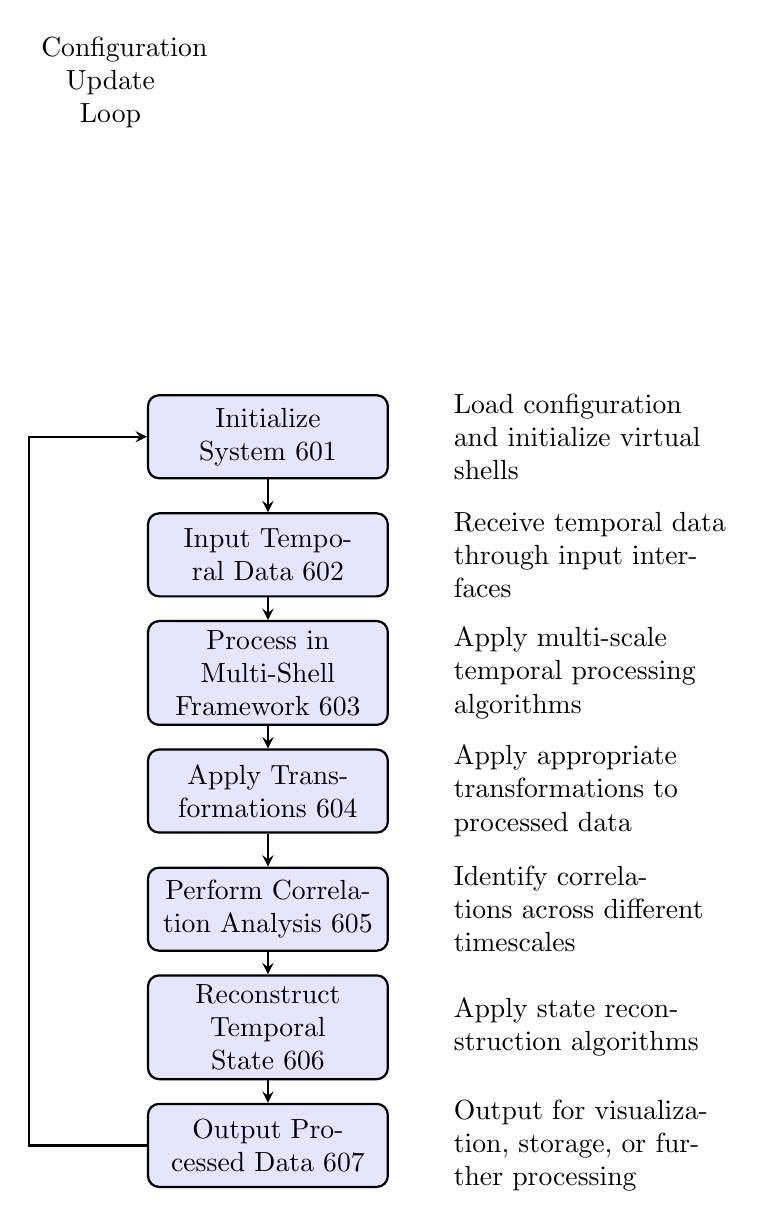
\begin{tikzpicture}[
    scale=1.0,
    block/.style={rectangle, draw, thick, fill=blue!10, text width=8em, text centered, rounded corners, minimum height=3em},
    line/.style={draw, ->, >=stealth, thick},
    ]
    
    % Define block positions
    \node[block] (init) at (0,0) {Initialize System 601};
    \node[block] (input) at (0,-1.5) {Input Temporal Data 602};
    \node[block] (process) at (0,-3) {Process in Multi-Shell Framework 603};
    \node[block] (transform) at (0,-4.5) {Apply Transformations 604};
    \node[block] (analyze) at (0,-6) {Perform Correlation Analysis 605};
    \node[block] (reconstruct) at (0,-7.5) {Reconstruct Temporal State 606};
    \node[block] (output) at (0,-9) {Output Processed Data 607};
    
    % Connect blocks with arrows
    \draw[line] (init) -- (input);
    \draw[line] (input) -- (process);
    \draw[line] (process) -- (transform);
    \draw[line] (transform) -- (analyze);
    \draw[line] (analyze) -- (reconstruct);
    \draw[line] (reconstruct) -- (output);
    
    % Add detail annotations
    \node[right=0.7cm of init, text width=10em, align=left] {Load configuration and initialize virtual shells};
    \node[right=0.7cm of input, text width=10em, align=left] {Receive temporal data through input interfaces};
    \node[right=0.7cm of process, text width=10em, align=left] {Apply multi-scale temporal processing algorithms};
    \node[right=0.7cm of transform, text width=10em, align=left] {Apply appropriate transformations to processed data};
    \node[right=0.7cm of analyze, text width=10em, align=left] {Identify correlations across different timescales};
    \node[right=0.7cm of reconstruct, text width=10em, align=left] {Apply state reconstruction algorithms};
    \node[right=0.7cm of output, text width=10em, align=left] {Output for visualization, storage, or further processing};
    
    % Add a feedback loop
    \draw[line] (output.west) -- ++(-1.5,0) -- ++(0,9) -- (init.west);
    \node[text width=5em, align=center] at (-2,4.5) {Configuration\\Update\\Loop};
    
\end{tikzpicture}
\caption*{FIG. 8}
\end{figure}

\begin{figure}[h]
\centering
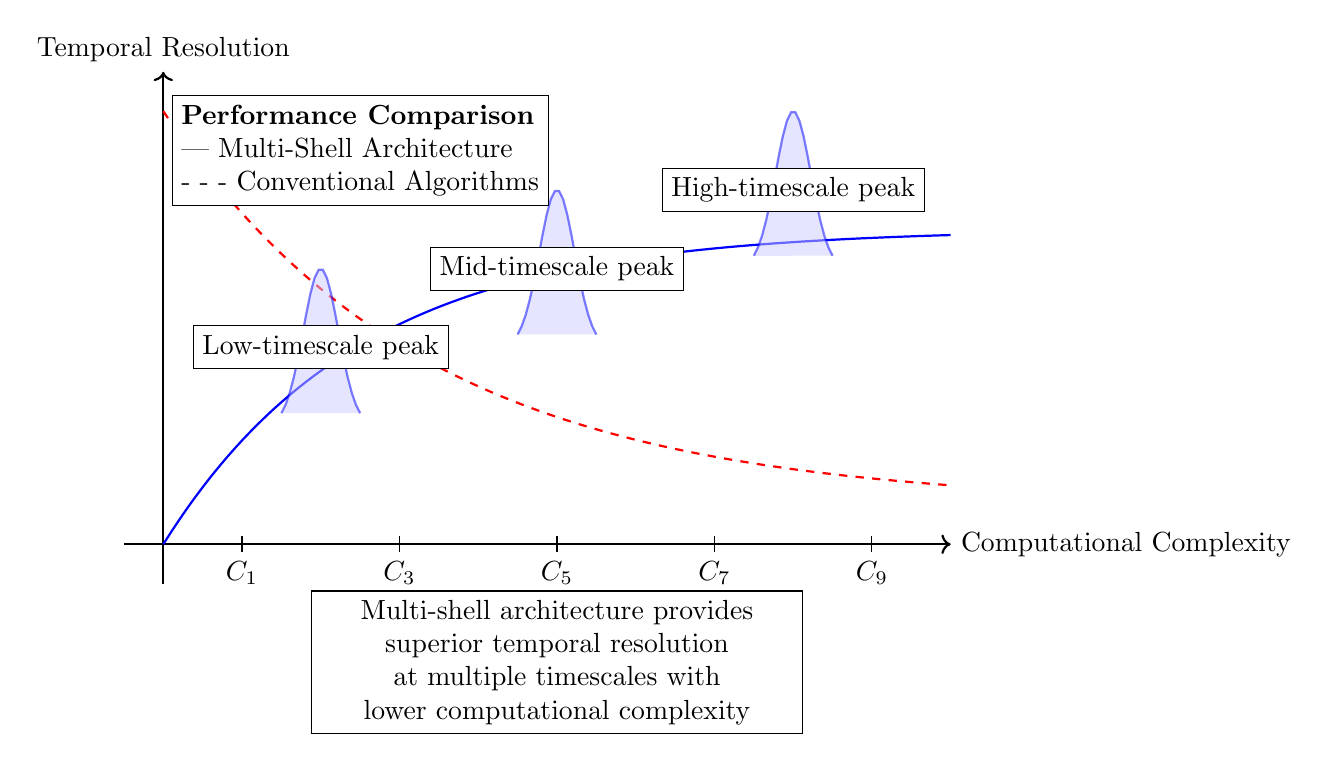
\begin{tikzpicture}[
    scale=1.0,
    axis/.style={thick, ->},
    conventional/.style={thick, dashed, red},
    multishell/.style={thick, blue},
    peak/.style={blue, thick, fill=blue!20, opacity=0.5},
    ]
    
    % Set up axes
    \draw[axis] (-0.5,0) -- (10,0) node[right] {Computational Complexity};
    \draw[axis] (0,-0.5) -- (0,6) node[above] {Temporal Resolution};
    
    % Add axis labels
    \foreach \x in {1,3,5,7,9} {
        \draw (\x,-0.1) -- (\x,0.1);
        \node[below] at (\x,-0.1) {$C_{\x}$};
    }
    
    % Draw conventional algorithm response curve (decreasing with complexity)
    \draw[conventional] plot[domain=0:10, samples=100] 
        (\x, {5*exp(-0.3*\x) + 0.5});
    
    % Draw multi-shell architecture response curve (increasing with complexity)
    \draw[multishell] plot[domain=0:10, samples=100] 
        (\x, {4*(1-exp(-0.4*\x))});
    
    % Draw resolution peaks for multi-shell architecture
    \draw[peak] plot[domain=1.5:2.5, samples=20] 
        (\x, {2*exp(-(\x-2)*(\x-2)/0.1) + 1.5});
    
    \draw[peak] plot[domain=4.5:5.5, samples=20] 
        (\x, {2*exp(-(\x-5)*(\x-5)/0.1) + 2.5});
    
    \draw[peak] plot[domain=7.5:8.5, samples=20] 
        (\x, {2*exp(-(\x-8)*(\x-8)/0.1) + 3.5});
    
    % Add labels
    \node[draw, fill=white, align=left] at (2.5,5) {
        \textbf{Performance Comparison}\\
        --- Multi-Shell Architecture\\
        - - - Conventional Algorithms
    };
    
    % Label the special features
    \node[draw, fill=white] at (2,2.5) {Low-timescale peak};
    \node[draw, fill=white] at (5,3.5) {Mid-timescale peak};
    \node[draw, fill=white] at (8,4.5) {High-timescale peak};
    
    % Add efficiency note
    \node[draw, fill=white!90, text width=6cm, align=center] at (5,-1.5) {
        Multi-shell architecture provides superior temporal resolution\\
        at multiple timescales with lower computational complexity
    };
    
\end{tikzpicture}
\caption*{FIG. 9}
\end{figure}

\begin{figure}[h]
\centering
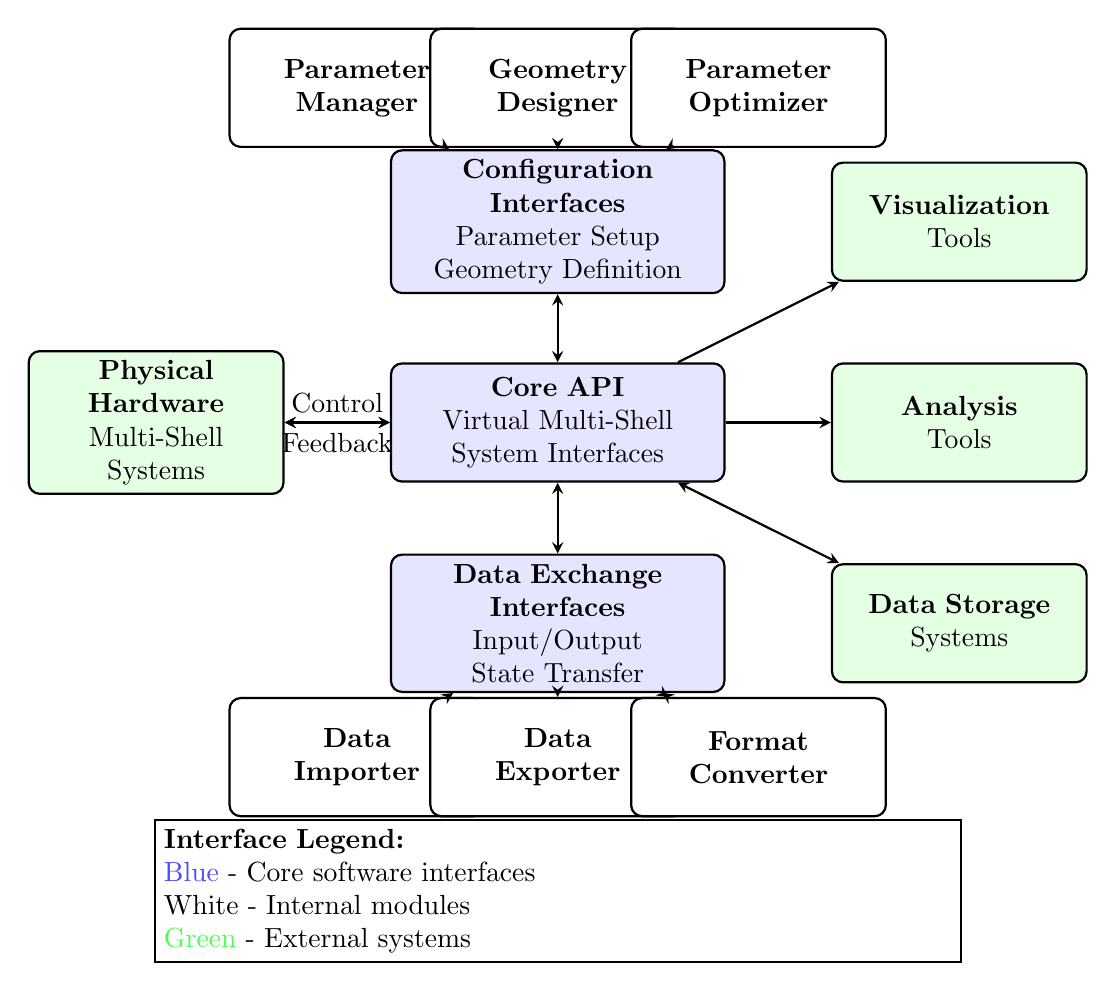
\begin{tikzpicture}[
    scale=0.85,
    interface/.style={rectangle, draw, thick, fill=blue!10, rounded corners, text width=4cm, align=center, minimum height=1.5cm},
    module/.style={rectangle, draw, thick, fill=white, rounded corners, text width=3cm, align=center, minimum height=1.5cm},
    external/.style={rectangle, draw, thick, fill=green!10, rounded corners, text width=3cm, align=center, minimum height=1.5cm},
    arrow/.style={->, >=stealth, thick},
    bidirectional/.style={<->, >=stealth, thick},
    ]
    
    % Core system
    \node[interface] (core) at (0,0) {\textbf{Core API}\\Virtual Multi-Shell\\System Interfaces};
    
    % Configuration interfaces
    \node[interface] (config) at (0,3) {\textbf{Configuration Interfaces}\\Parameter Setup\\Geometry Definition};
    
    % Data exchange interfaces
    \node[interface] (data) at (0,-3) {\textbf{Data Exchange Interfaces}\\Input/Output\\State Transfer};
    
    % External systems
    \node[external] (hardware) at (-6,0) {\textbf{Physical Hardware}\\Multi-Shell\\Systems};
    \node[external] (visualization) at (6,3) {\textbf{Visualization}\\Tools};
    \node[external] (analysis) at (6,0) {\textbf{Analysis}\\Tools};
    \node[external] (storage) at (6,-3) {\textbf{Data Storage}\\Systems};
    
    % Specific modules
    \node[module] (param) at (-3,5) {\textbf{Parameter\\Manager}};
    \node[module] (geom) at (0,5) {\textbf{Geometry\\Designer}};
    \node[module] (optimizer) at (3,5) {\textbf{Parameter\\Optimizer}};
    
    \node[module] (importer) at (-3,-5) {\textbf{Data\\Importer}};
    \node[module] (exporter) at (0,-5) {\textbf{Data\\Exporter}};
    \node[module] (converter) at (3,-5) {\textbf{Format\\Converter}};
    
    % Connect interfaces to core
    \draw[bidirectional] (core) -- (config);
    \draw[bidirectional] (core) -- (data);
    
    % Connect configuration modules
    \draw[arrow] (param) -- (config);
    \draw[arrow] (geom) -- (config);
    \draw[arrow] (optimizer) -- (config);
    
    % Connect data exchange modules
    \draw[arrow] (importer) -- (data);
    \draw[arrow] (data) -- (exporter);
    \draw[arrow] (converter) -- (data);
    \draw[arrow] (data) -- (converter);
    
    % Connect external systems
    \draw[bidirectional] (core) -- (hardware) node[midway, above] {Control};
    \draw[bidirectional] (core) -- (hardware) node[midway, below] {Feedback};
    
    \draw[arrow] (core) -- (analysis);
    \draw[arrow] (core) -- (visualization);
    \draw[bidirectional] (core) -- (storage);
    
    % Add legend
    \node[draw, thick, fill=white, text width=10cm, align=left] at (0,-7) {
        \textbf{Interface Legend:}\\
        \textcolor{blue!70}{Blue} - Core software interfaces\\
        \textcolor{black}{White} - Internal modules\\
        \textcolor{green!70}{Green} - External systems
    };
    
\end{tikzpicture}
\caption*{FIG. 10}
\end{figure}

\end{document}